\documentclass[11pt]{article}

\usepackage[margin=0.78in]{geometry}
\usepackage{graphicx}
\usepackage{xcolor}
\usepackage{microtype}
\usepackage{parskip}
\usepackage{hyperref}
\usepackage{pagecolor}

\definecolor{ink}{HTML}{17202A}
\definecolor{blue}{HTML}{146C94}
\definecolor{gold}{HTML}{D9942B}
\definecolor{paper}{HTML}{F7F4EE}
\definecolor{muted}{HTML}{5D6872}

\pagecolor{paper}
\color{ink}
\hypersetup{colorlinks=true,urlcolor=blue}
\setlength{\parindent}{0pt}
\pagestyle{empty}

\newcommand{\sectiontag}[1]{\vspace{0.2em}{\sffamily\bfseries\large\color{blue}#1}\par\vspace{0.35em}}
\newcommand{\ruleline}{\textcolor{gold}{\rule{\linewidth}{1.2pt}}}

\begin{document}

{\sffamily\color{blue}\large A LinkedIn introduction to SEFI}\par
\vspace{0.25em}
{\sffamily\bfseries\fontsize{28}{31}\selectfont One entity. Two directions.\par\vspace{0.1em}One very different way to picture a particle.}\par
\vspace{0.55em}
\ruleline
\vspace{0.85em}

{\large
What if the electron and the positron are not two unrelated things, but two orientations of one continuous entity?}

That is the starting intuition behind my unified geometric field theory.

In the model, a particle is not imagined as a tiny billiard ball with a permanent label stuck to it. It is represented by a worldline: a geometric path through spacetime. Change the orientation of that path, and the same underlying entity can appear in what we conventionally call the electron and positron sectors.

The picture is simple enough to explain over coffee, but ambitious enough to keep the coffee awake:

\begin{center}
{\sffamily\bfseries\large one entity + different orientation = different observed sector}
\end{center}

The larger framework connects worldline geometry with identity-space dynamics, stability surfaces, and photonic error correction. The goal is not to replace established quantum field theory by declaration. It is to offer a geometric lens for asking whether some familiar distinctions are properties of the entity itself, or properties of how its trajectory is oriented and observed.

The four images in this short introduction move from photonic implementation, to worldline geometry, to the stability surface, and finally to observer geometry: the idea that the structure of observation can generate useful quantum intuition before the full mathematics arrives.

\vfill
{\sffamily\bfseries\color{blue}The short version:}\par
\vspace{0.25em}
{\large We may be looking at one continuous story and naming its directions as different particles.}

\vfill
{\sffamily\color{muted}\small Unified Geometric Field Theory / GWFM / SEFI / DEFI}\par
\newpage

\sectiontag{01 / Photonic intuition}
{\sffamily\bfseries\fontsize{23}{26}\selectfont Start with a system that makes correlation visible.}\par
\vspace{0.45em}
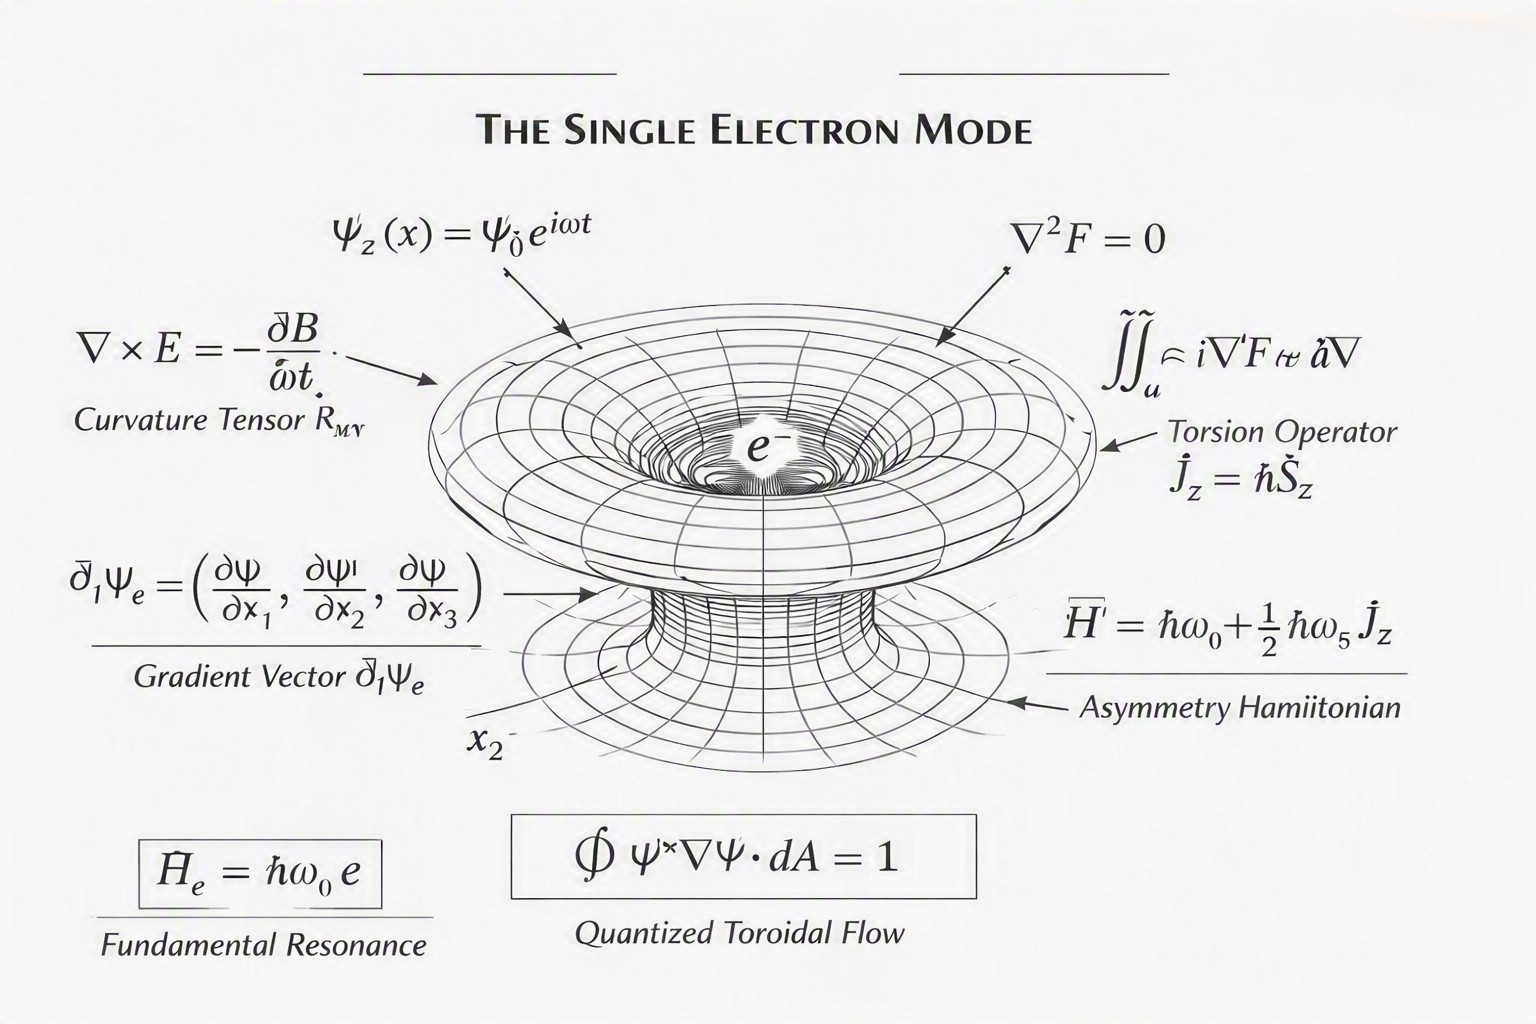
\includegraphics[width=0.98\linewidth,height=5.1in,keepaspectratio]{Fig5_Photonic_Implementation.jpg}
\vspace{0.35em}

Photonic systems give the idea a friendly entry point. Paths, correlations, stabilizers, and measured deviations can be drawn before they are buried under notation. The geometry is doing something practical here: it tells us what counts as a stable pattern, what counts as a deviation, and what a correction is supposed to restore.

The same design language then travels inward, from an optical setup to the geometry of a single entity moving through spacetime.
\newpage

\sectiontag{02 / One worldline}
{\sffamily\bfseries\fontsize{23}{26}\selectfont The particle is the path, not a tiny passenger on the path.}\par
\vspace{0.45em}
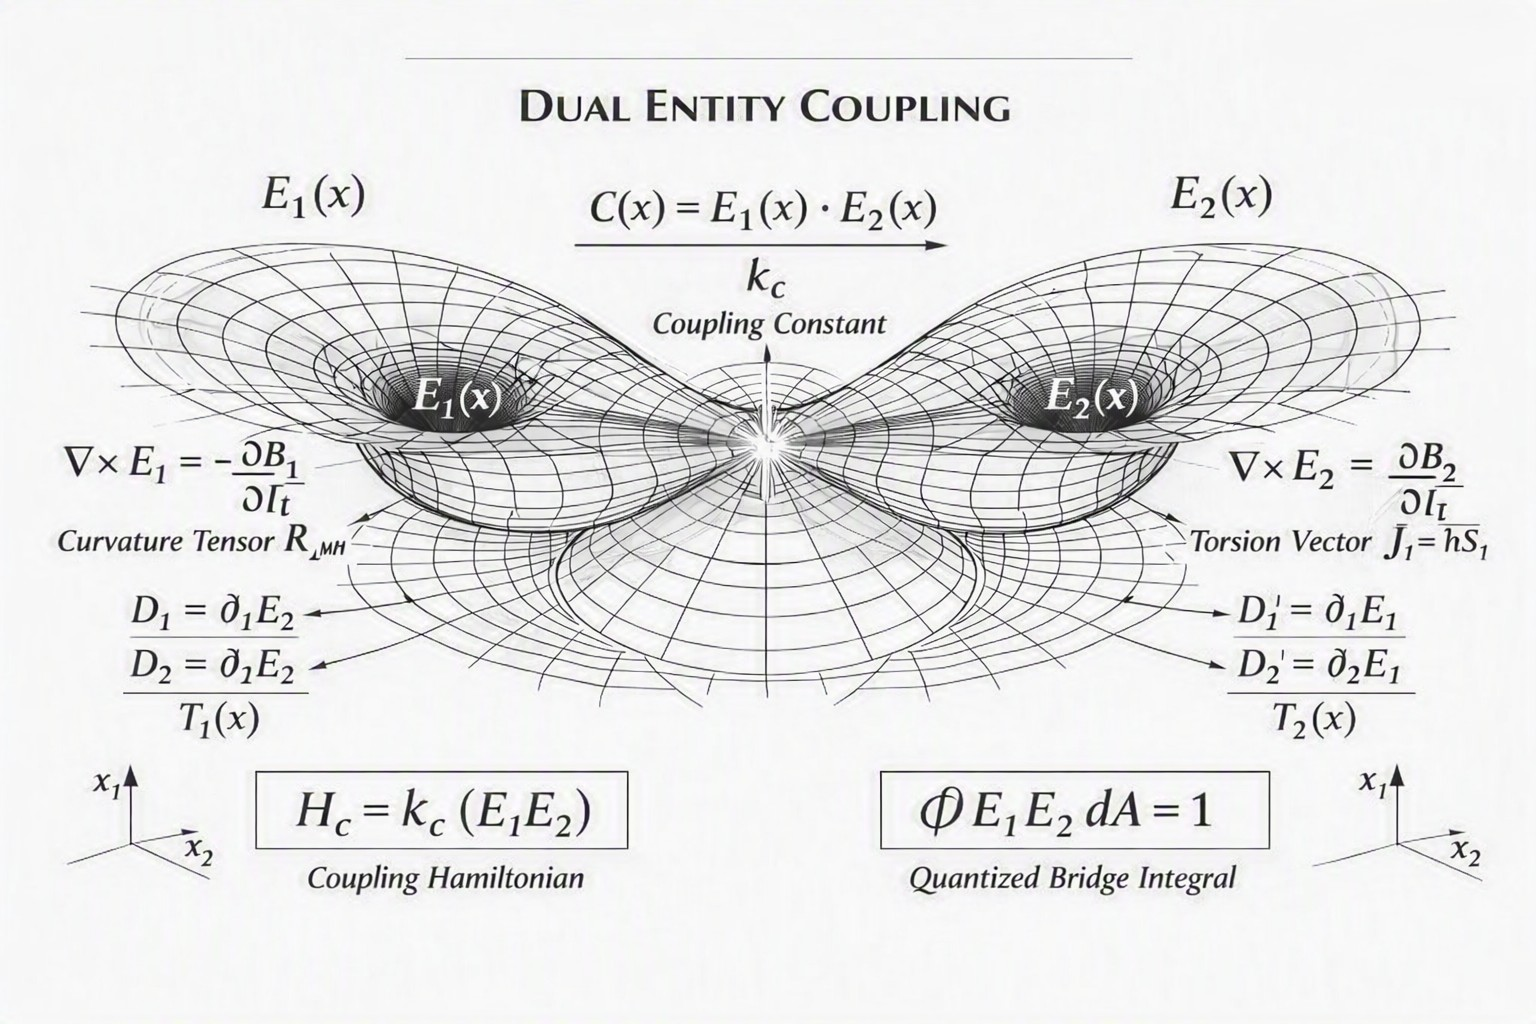
\includegraphics[width=0.98\linewidth,height=5.05in,keepaspectratio]{Fig2_Worldline_Geometry.jpg}
\vspace{0.35em}

Here the basic object is a worldline with geometric features: curvature, torsion, direction, and continuity. In the proposed framework, these are not decorative details. They are part of the information carried by the entity.

Now reverse the orientation of the story. The proposal is that the forward-time and backward-time sectors conventionally associated with electron and positron behavior can be understood as different orientations of the same underlying entity.
\newpage

\sectiontag{03 / The stability surface}
{\sffamily\bfseries\fontsize{23}{26}\selectfont Two appearances, one geometric home.}\par
\vspace{0.45em}
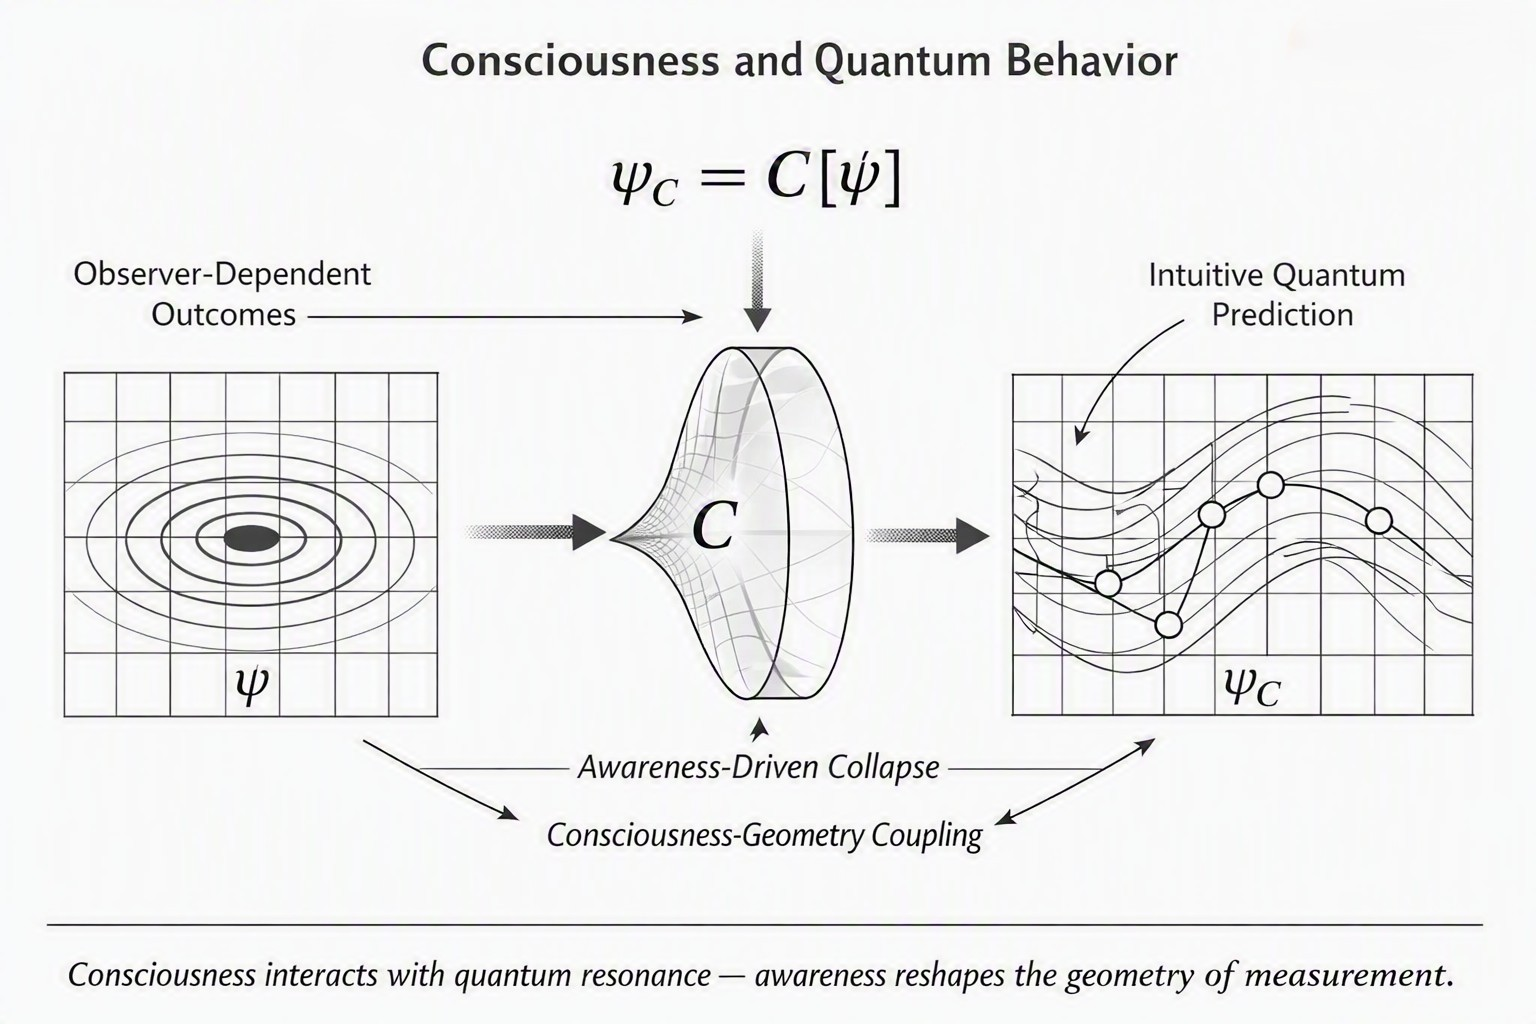
\includegraphics[width=0.98\linewidth,height=5.05in,keepaspectratio]{Fig1_Stability_Surface.jpg}
\vspace{0.35em}

A stability surface is the model's way of saying: these geometric and identity conditions belong together. The electron and positron are not being glued together by wordplay; they are being placed in one larger state-space picture, where orientation and invariants matter.

That does not make the interpretation experimentally settled. It does make the question precise enough to calculate with, compare with known physics, and eventually test.
\newpage

\sectiontag{04 / Observer geometry}
{\sffamily\bfseries\fontsize{23}{26}\selectfont Quantum intuition may begin with where we stand.}\par
\vspace{0.45em}
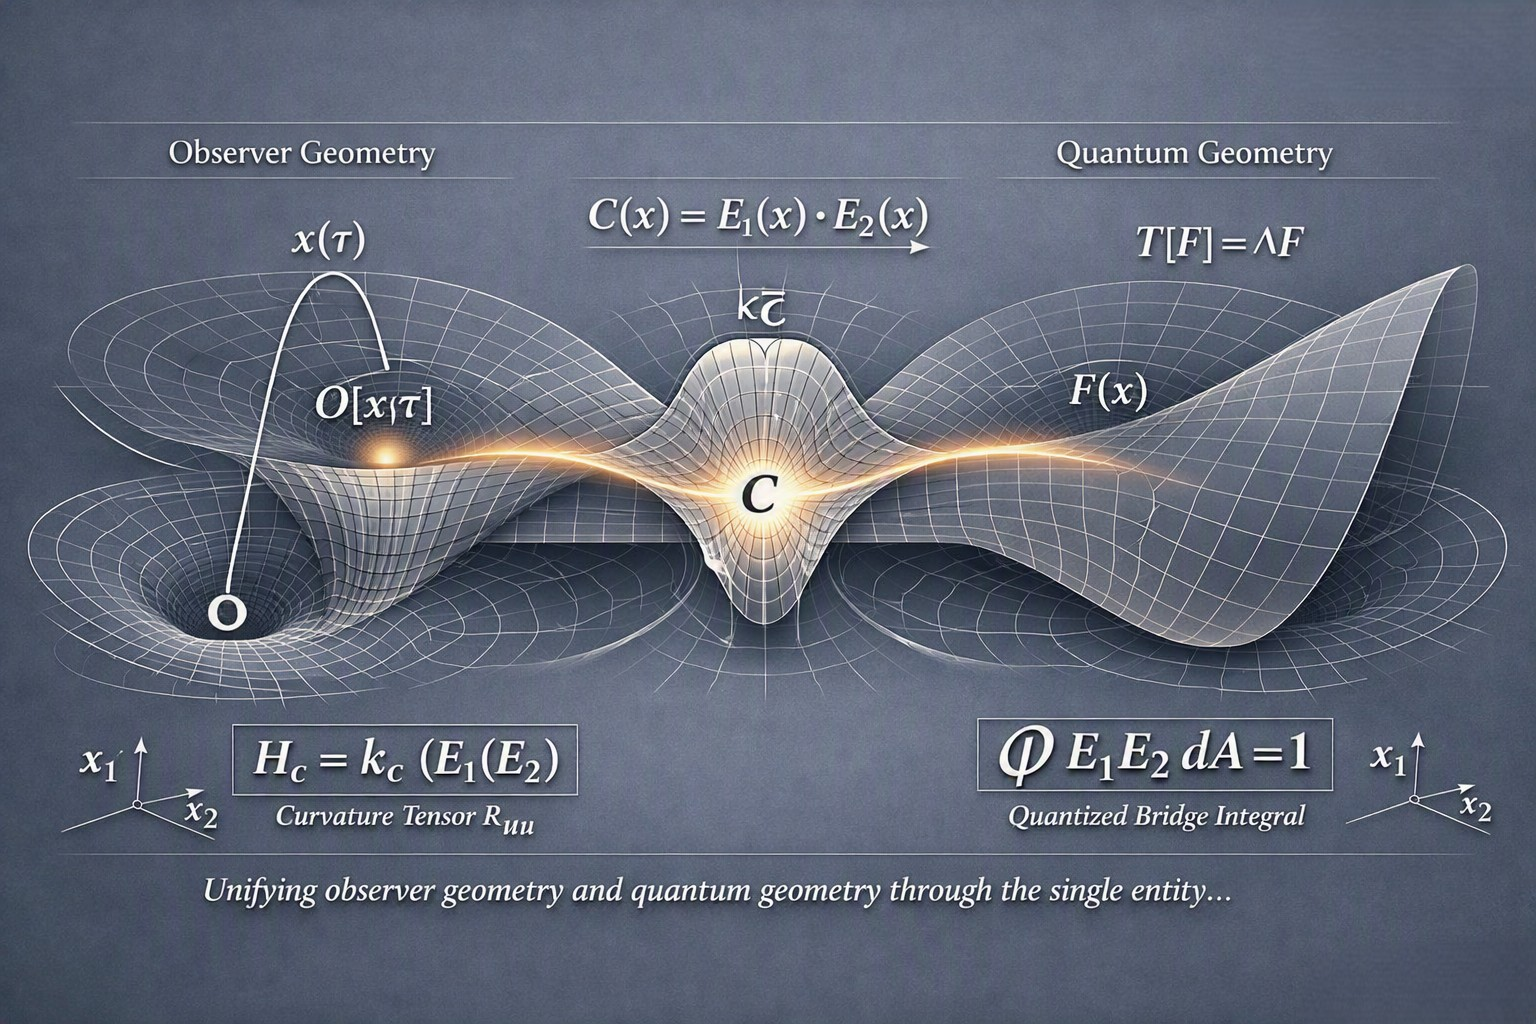
\includegraphics[width=0.98\linewidth,height=5.05in,keepaspectratio]{Highlight.jpg}
\vspace{0.35em}

The final step is the most philosophical, and possibly the most useful: an observation is never just a passive window. It has geometry. It selects a direction, a frame, a decomposition, and a set of invariants that can be measured.

In this view, quantum intuition emerges when the geometry of the observer and the geometry of the entity meet. What looks like two particles may be one entity seen through two orientations. What looks like an error may be displacement from a stability surface. What looks mysterious may be a coordinate choice we have not yet learned to see.

That is the invitation of the work: keep the mathematics rigorous, keep the intuition human, and ask better questions about what a particle is before deciding how many things we are looking at.

\vfill
{\sffamily\bfseries\color{blue}This is the opening intuition. The full theory develops the operator, invariants, stability manifolds, correction mapping, and cosmological extension.}\par
\vspace{0.3em}
{\sffamily\color{muted}\small Jason Duran Dutton / Castlewood, Virginia}\par

\end{document}
